\section{Sample System Ouput - Filtered Data}
This section contains filtered states required to estimate a drag polar.
\begin{figure}[]
	\centering
	\caption{qbar vs. Time}
		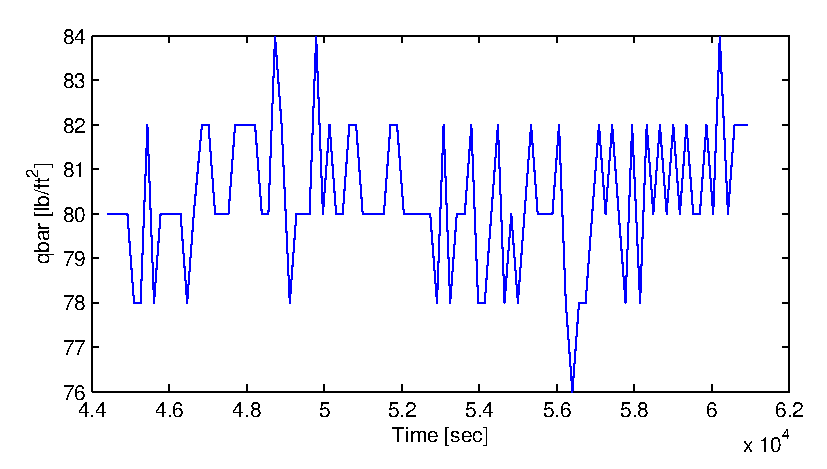
\includegraphics[width = 0.7\textwidth]{C:/Users/mufasa/Documents/Thesis/LaTex/figures/sampleOutput/Filtered/qbar.eps}
\end{figure}
\begin{figure}[]
	\centering
	\caption{rho vs. Time}
		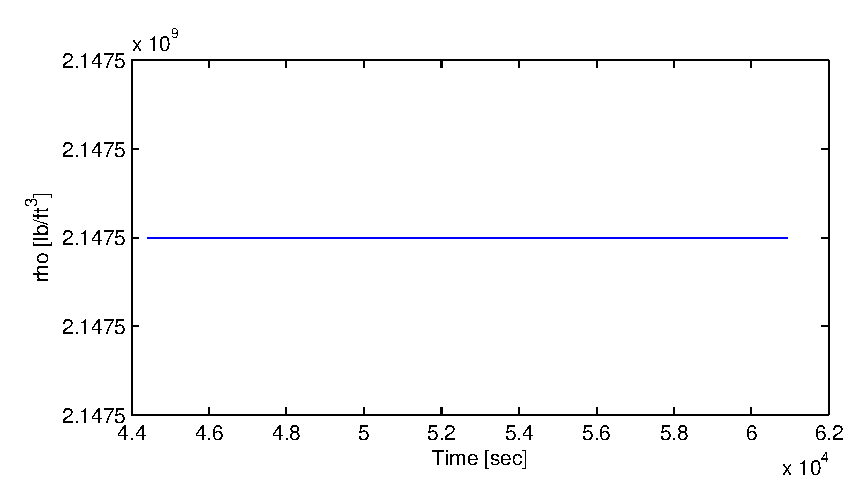
\includegraphics[width = 0.7\textwidth]{C:/Users/mufasa/Documents/Thesis/LaTex/figures/sampleOutput/Filtered/rho.eps}
\end{figure}
\clearpage
\begin{figure}[]
	\centering
	\caption{alpha vs. Time}
		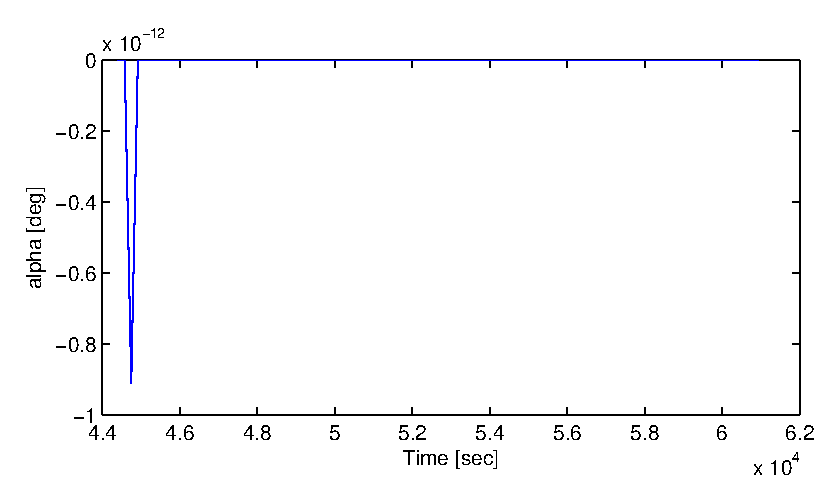
\includegraphics[width = 0.7\textwidth]{C:/Users/mufasa/Documents/Thesis/LaTex/figures/sampleOutput/Filtered/alpha.eps}
\end{figure}
\begin{figure}[]
	\centering
	\caption{beta vs. Time}
		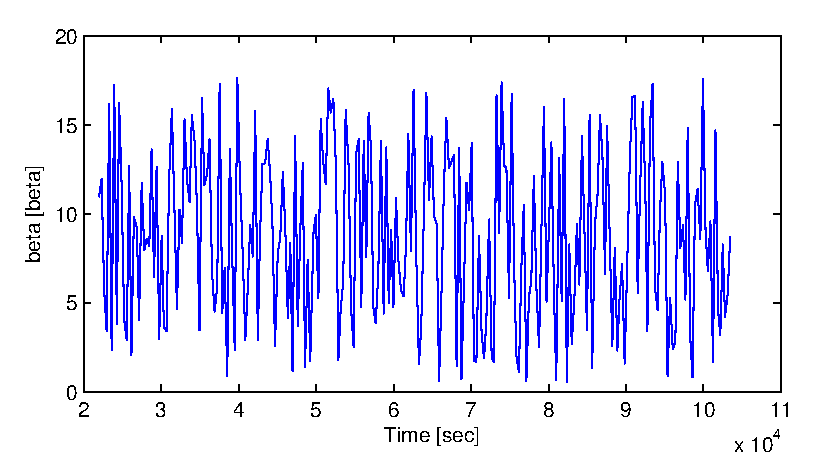
\includegraphics[width = 0.7\textwidth]{C:/Users/mufasa/Documents/Thesis/LaTex/figures/sampleOutput/Filtered/beta.eps}
\end{figure}
\begin{figure}[]
	\centering
	\caption{roll vs. Time}
		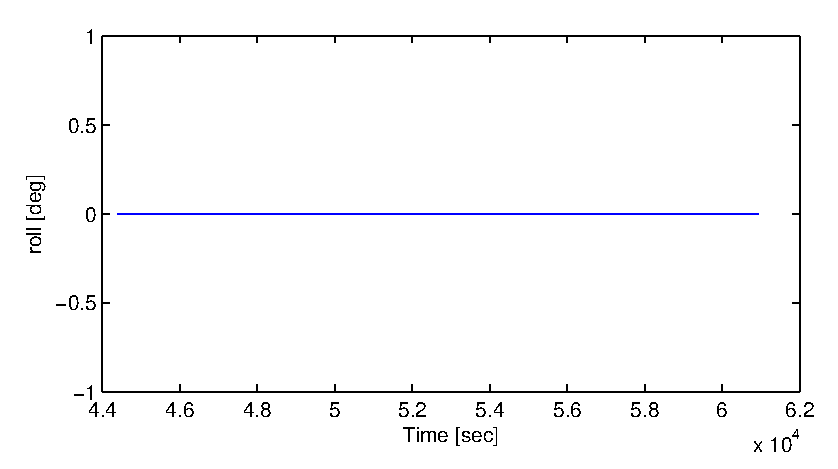
\includegraphics[width = 0.7\textwidth]{C:/Users/mufasa/Documents/Thesis/LaTex/figures/sampleOutput/Filtered/roll.eps}
\end{figure}
\begin{figure}[]
	\centering
	\caption{pitch vs. Time}
		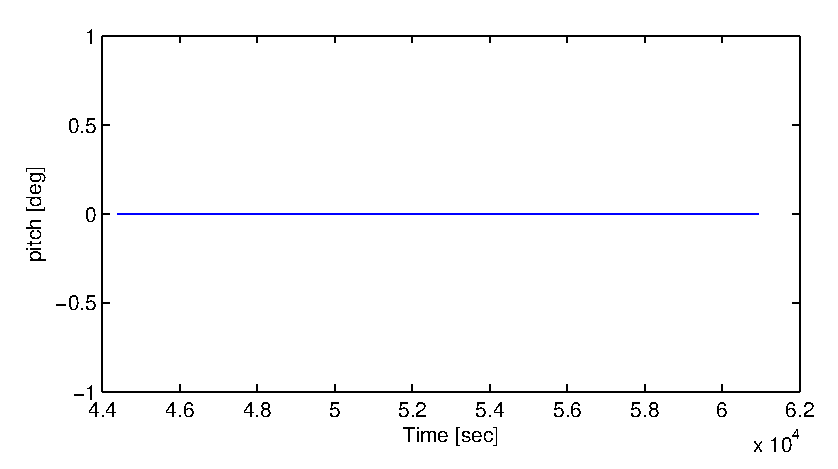
\includegraphics[width = 0.7\textwidth]{C:/Users/mufasa/Documents/Thesis/LaTex/figures/sampleOutput/Filtered/pitch.eps}
\end{figure}
\begin{figure}[]
	\centering
	\caption{yaw vs. Time}
		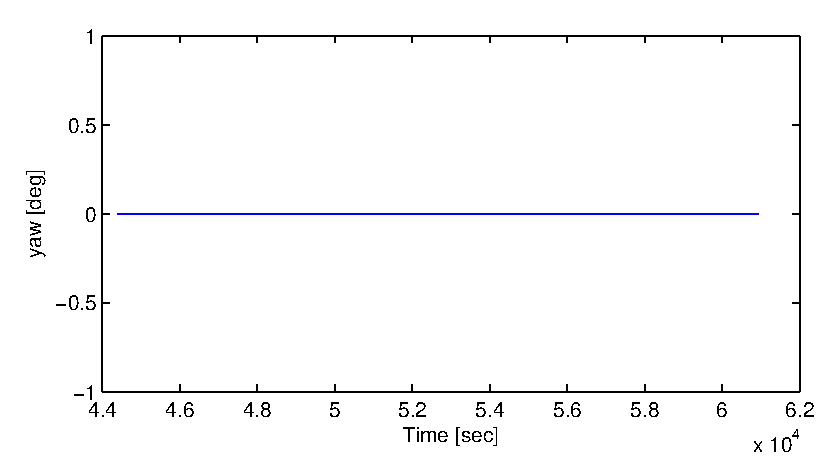
\includegraphics[width = 0.7\textwidth]{C:/Users/mufasa/Documents/Thesis/LaTex/figures/sampleOutput/Filtered/yaw.eps}
\end{figure}
\begin{figure}[]
	\centering
	\caption{rollRate vs. Time}
		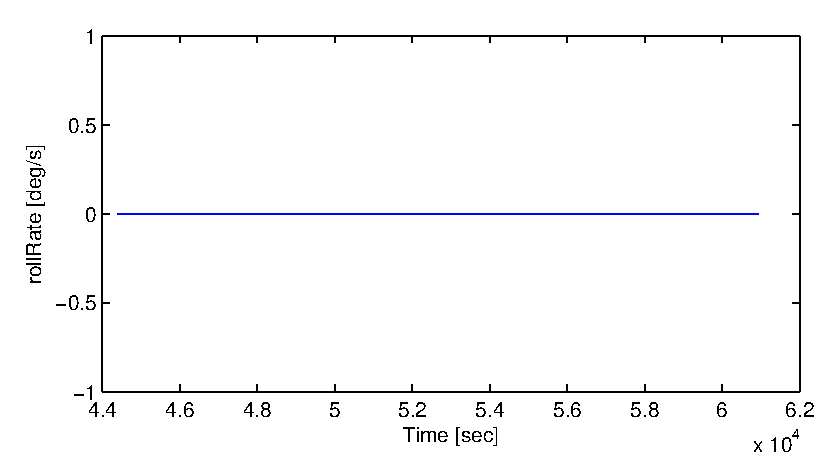
\includegraphics[width = 0.7\textwidth]{C:/Users/mufasa/Documents/Thesis/LaTex/figures/sampleOutput/Filtered/rollRate.eps}
\end{figure}
\begin{figure}[]
	\centering
	\caption{pitchRate vs. Time}
		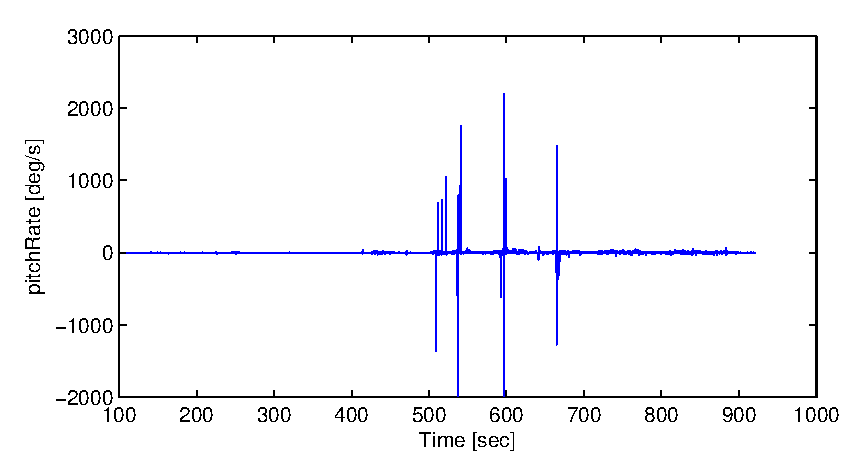
\includegraphics[width = 0.7\textwidth]{C:/Users/mufasa/Documents/Thesis/LaTex/figures/sampleOutput/Filtered/pitchRate.eps}
\end{figure}
\begin{figure}[]
	\centering
	\caption{yawRate vs. Time}
		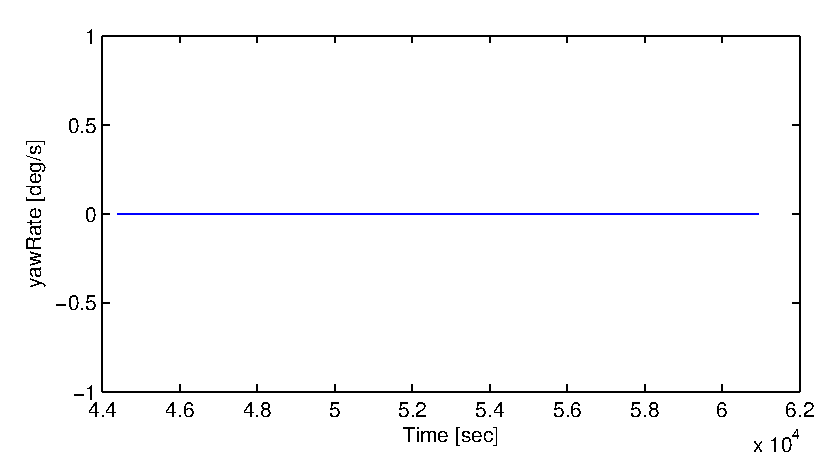
\includegraphics[width = 0.7\textwidth]{C:/Users/mufasa/Documents/Thesis/LaTex/figures/sampleOutput/Filtered/yawRate.eps}
\end{figure}
\begin{figure}[]
	\centering
	\caption{accelX vs. Time}
		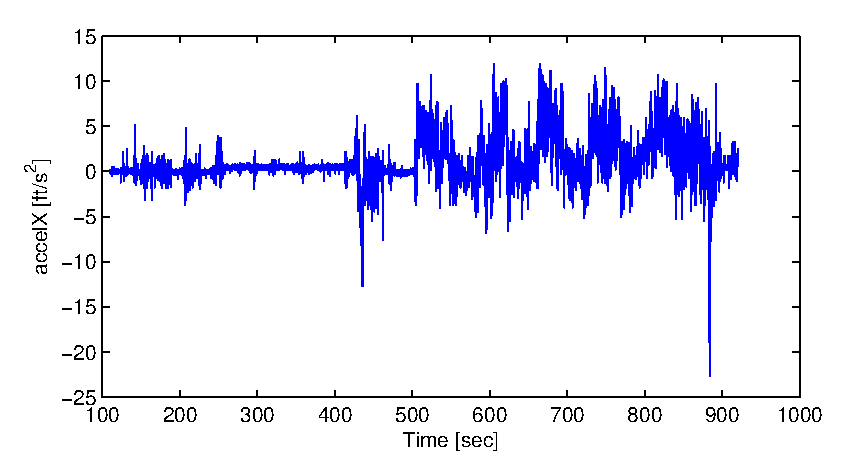
\includegraphics[width = 0.7\textwidth]{C:/Users/mufasa/Documents/Thesis/LaTex/figures/sampleOutput/Filtered/accelX.eps}
\end{figure}
\begin{figure}[]
	\centering
	\caption{accelY vs. Time}
		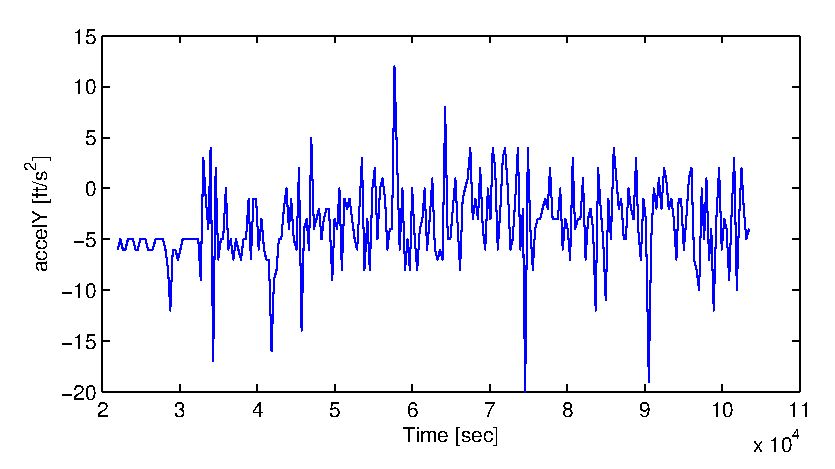
\includegraphics[width = 0.7\textwidth]{C:/Users/mufasa/Documents/Thesis/LaTex/figures/sampleOutput/Filtered/accelY.eps}
\end{figure}
\begin{figure}[]
	\centering
	\caption{accelZ vs. Time}
		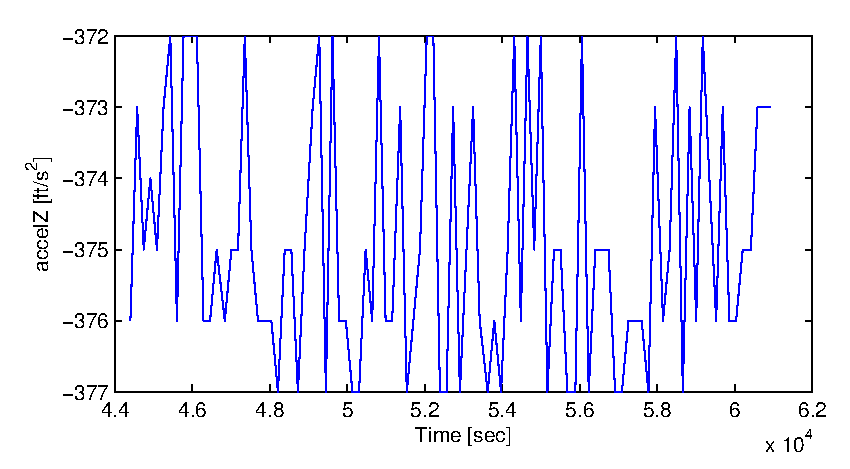
\includegraphics[width = 0.7\textwidth]{C:/Users/mufasa/Documents/Thesis/LaTex/figures/sampleOutput/Filtered/accelZ.eps}
\end{figure}
